%!TEX root = ../../main.tex
% ============================================================
% 几何作图 / 图形规律与序列
% 本文件由 main.tex 通过 \input 引入，请勿单独编译
% 重构日期: 2026-04-11
% ============================================================

\subsection{gpt-5.2-codex}

\begin{tikzpicture}[scale=1]
% 第一条：1/3
\draw (0,0) rectangle (6,1);
\foreach \x in {2,4} {
  \draw (\x,0) -- (\x,1);
}
\fill[gray!40] (0,0) rectangle (2,1);
\node at (3,-0.4) {$\dfrac{1}{3}$};
% 第二条：1/4
\draw (0,-2) rectangle (6,-1);
\foreach \x in {1.5,3,4.5} {
  \draw (\x,-2) -- (\x,-1);
}
\fill[gray!40] (0,-2) rectangle (1.5,-1);
\node at (3,-2.4) {$\dfrac{1}{4}$};
% 大于号
\node at (7, -1) {\Large $>$};
\end{tikzpicture}

\newpage

\subsection{gpt-5.4}

\begin{tikzpicture}[scale=1]
% 上面：1/3
\draw (0,2) rectangle (9,3);
\draw (3,2) -- (3,3);
\draw (6,2) -- (6,3);
\fill[blue!30] (0,2) rectangle (3,3);
\node[left] at (0,2.5) {$\frac{1}{3}$};
% 下面：1/4
\draw (0,0) rectangle (9,1);
\draw (2.25,0) -- (2.25,1);
\draw (4.5,0) -- (4.5,1);
\draw (6.75,0) -- (6.75,1);
\fill[red!30] (0,0) rectangle (2.25,1);
\node[left] at (0,0.5) {$\frac{1}{4}$};
% 说明文字
\node at (4.5,-0.8) {同样大的整体，平均分成的份数越多，每一份越小。};
\node at (4.5,-1.5) {所以 $\frac{1}{3}>\frac{1}{4}$。};
\end{tikzpicture}


%% ==============================
%% 黑板报版面比例问题 (1/3, 1/3, 1/6, 1/6)
%% ==============================


\newpage

\begin{center}
  {\large\bfseries 解答：黑板报版面比例问题}
\end{center}

\vspace{0.6cm}

\noindent
{\small \textbf{题目要求：} 新学期三(2)班的黑板报一共设置了四个栏目。其中，“知识窗”占黑板报的 $\frac{1}{3}$，剩下的 $\frac{1}{2}$ 为“科学园地”，“安全角”和“新学期寄语”各占了最后剩下的一半。“安全角”和“新学期寄语”各占黑板报的几分之几？（先在图中画一画，再回答。）}

\vspace{1.0cm}

\begin{center}
  \begin{tikzpicture}[scale=1.5, >=Stealth]
    % 定义黑板总尺寸
    \def\totalW{6}
    \def\totalH{4}

    % --- 绘制各区域并填充颜色 ---
    
    % 1. 知识窗 (占 1/3) -> 6 * 1/3 = 2 cm 宽
    \fill[cyan!20] (0, 0) rectangle (2, \totalH);
    \draw[cyan!70!blue, line width=1pt] (0,0) rectangle (2, \totalH);
    \node[align=center] at (1, 0.5*\totalH) {\small 知识窗 \\ $\frac{1}{3}$};

    % 2. 科学园地 (占剩余 2/3 的一半，即 1/3) -> 2 cm 宽
    \fill[green!20] (2, 0) rectangle (4, \totalH);
    \draw[green!60!black, line width=1pt] (2,0) rectangle (4, \totalH);
    \node[align=center] at (3, 0.5*\totalH) {\small 科学园地 \\ $\frac{1}{3}$};

    % 3. 安全角 (占最后 1/3 的一半，即 1/6) -> 2 cm 宽, 对半高度
    \fill[yellow!30] (4, 2) rectangle (6, \totalH);
    \draw[orange!80!black, line width=1pt] (4, 2) rectangle (6, \totalH);
    \node[align=center] at (5, 3) {\small 安全角 \\ $\frac{1}{6}$};

    % 4. 新学期寄语 (占最后 1/3 的一半，即 1/6)
    \fill[orange!20] (4, 0) rectangle (6, 2);
    \draw[orange!80!black, line width=1pt] (4, 0) rectangle (6, 2);
    \node[align=center] at (5, 1) {\small 新学期寄语 \\ $\frac{1}{6}$};

    % --- 整体边框 ---
    \draw[cyan!70!blue, line width=1.2pt] (0, 0) rectangle (\totalW, \totalH);

  \end{tikzpicture}
\end{center}

\vspace{1.0cm}
\hrule
\vspace{0.4cm}

% 说明与回答
{\small
\textbf{逻辑推算与解答：} \\
1. \textbf{第一步}：“知识窗”占黑板报的 $\frac{1}{3}$。 \\
2. \textbf{第二步}：剩下的部分占黑板报的 $1 - \frac{1}{3} = \frac{2}{3}$。 \\
3. \textbf{第三步}：“科学园地”占剩下部分的 $\frac{1}{2}$，即 $\frac{2}{3} \times \frac{1}{2} = \frac{1}{3}$。 \\
4. \textbf{第四步}：最后剩下的部分占黑板报的 $\frac{2}{3} - \frac{1}{3} = \frac{1}{3}$。 \\
5. \textbf{第五步}：“安全角”和“新学期寄语”平分最后剩下的 $\frac{1}{3}$，即 $\frac{1}{3} \div 2 = \frac{1}{6}$。 \\

\textbf{答案：}“安全角”和“新学期寄语”各占黑板报的 \textbf{$\frac{1}{6}$}。
}


%% ==============================
%% 两位数乘法的面积模型 (45 x 36)
%% ==============================


\newpage

\begin{center}
  {\large\bfseries 解答：两位数乘法的面积模型}
\end{center}

\vspace{0.6cm}

\noindent
{\small \textbf{题目要求：} 先算一算，再在图中标出每一步计算的结果。}

\vspace{1.0cm}

\begin{center}
  \begin{minipage}{0.4\textwidth}
    \centering
    \textbf{竖式计算：}
    \vspace{0.5cm}
    
    {\Large
    \begin{tabular}{r@{\,}r@{\,}r@{\,}r@{\,}r@{\,}r}
      & & & & 4 & 5 \\
      $\times$ & & & & 3 & 6 \\
      \hline
      & & & 2 & 7 & 0 \\
      & & 1 & 3 & 5 & 0 \\
      \hline
      & & 1 & 6 & 2 & 0 \\
    \end{tabular}
    }
  \end{minipage}
  \hfill
  \begin{minipage}{0.55\textwidth}
    \centering
    \textbf{面积模型说明：}
    \vspace{0.5cm}

    \begin{tikzpicture}[scale=0.8, >=Stealth]
      % 使用 pgfmathsetmacro 确保算术正常展开
      \pgfmathsetmacro{\wA}{4.0}
      \pgfmathsetmacro{\wB}{1.0}
      \pgfmathsetmacro{\hA}{3.0}
      \pgfmathsetmacro{\hB}{1.0}
      \pgfmathsetmacro{\wTotal}{\wA+\wB}
      \pgfmathsetmacro{\hTotal}{\hA+\hB}
      \pgfmathsetmacro{\wAhalf}{0.5*\wA}
      \pgfmathsetmacro{\wBcen}{\wA+0.5*\wB}
      \pgfmathsetmacro{\hBhalf}{0.5*\hB}
      \pgfmathsetmacro{\hAcen}{\hB+0.5*\hA}

      % --- 绘制并填充分割区域 ---
      \draw[cyan!70!blue, line width=1.2pt] (0, 0) rectangle (\wTotal, \hTotal);
      \draw[cyan!70!blue, line width=1pt] (0, \hB) -- (\wTotal, \hB);
      \draw[cyan!70!blue, line width=1pt] (\wA, 0) -- (\wA, \hTotal);

      % --- 外部标注 ---
      \node[above] at (\wAhalf, \hTotal) {\normalsize 40};
      \node[above] at (\wBcen, \hTotal) {\normalsize 5};
      \node[left] at (0, \hAcen) {\normalsize 30};
      \node[left] at (0, \hBhalf) {\normalsize 6};

      % --- 内部标注 (每一步计算结果, 使用小字号) ---
      \node at (\wAhalf, \hAcen) {\small \textbf{1200}};  % 40 * 30
      \node at (\wBcen, \hAcen) {\small \textbf{150}};    % 5 * 30
      \node at (\wAhalf, \hBhalf) {\small \textbf{240}};  % 40 * 6
      \node at (\wBcen, \hBhalf) {\small \textbf{30}};    % 5 * 6

    \end{tikzpicture}
  \end{minipage}
\end{center}

\vspace{1.0cm}
\hrule
\vspace{0.4cm}

% 解析
{\small
\textbf{解题思路：} \\
1. \textbf{拆分乘数}：根据位置原则，将 $45$ 拆分为 $40 + 5$，将 $36$ 拆分为 $30 + 6$。 \\
2. \textbf{分步计算}：利用乘法分配律，分别计算四个部分的面积： \\
   - $40 \times 30 = 1200$ \\
   - $5 \times 30 = 150$ \\
   - $40 \times 6 = 240$ \\
   - $5 \times 6 = 30$ \\
3. \textbf{汇总求和}：将四个部分的结果相加：$1200 + 150 + 240 + 30 = 1620$。 \\
这与竖式计算中 $1350 (45 \times 30) + 270 (45 \times 6) = 1620$ 的结果是一致的。
}


%% ==============================
%% 第 3 题：画 35° 角；利用垂直线画长方形
%% ==============================

\newpage

\newpage

\begin{center}
  {\large\bfseries 解答：周期规律图形序列}
\end{center}

\vspace{0.6cm}

\noindent{\small \textbf{题目信息：}}\\
{\small 小亮设计的图形序列：$\bigcirc \bigcirc \square \star \bigcirc \bigcirc \square \star \bigcirc \bigcirc \square \star \bigcirc \cdots\cdots$}

\vspace{0.8cm}
\hrule
\vspace{0.5cm}

{\small
\textbf{(1)} 根据小亮的设计，第 30 个图形是（\quad \textbf{$\bigcirc$} \quad）。

\vspace{0.3cm}
\textit{分析：}\\
小亮的设计是由“$\bigcirc \bigcirc \square \star$”这 4 个图形作为一组循环出现的（即周期为 $4$）。\\
计算：$30 \div 4 = 7$（组）$\cdots\cdots 2$（个）。\\
余数为 $2$ ，表示第 $30$ 个图形与每组周期里的第 $2$ 个图形相同。\\
周期里第 $2$ 个图形是 $\bigcirc$，因此第 $30$ 个图形就是 $\bigcirc$。

\vspace{0.8cm}
\textbf{(2)} 小明想让第 30 个图形是 $\star$，他可以怎样设计？在横线上画一画。

\vspace{0.3cm}
\textit{设计图例：}\\
\underline{\quad \Large $\bigcirc$\quad$\square$\quad$\star$\quad$\bigcirc$\quad$\square$\quad$\star$\quad$\bigcirc$\quad$\square$\quad$\star$\quad$\cdots\cdots$ \quad}

\vspace{0.6cm}
\textit{分析：}\\
要让第 $30$ 个图形是 $\star$，意味着 $30$ 这个序号需要落在该周期序列中 $\star$ 所在的位置。\\
最简单的设计方案是：让周期数量为 $3$，并在每组的末尾放置 $\star$（即周期序列为“$\bigcirc\square\star$”）。\\
计算验证：$30 \div 3 = 10$（组）$\cdots\cdots 0$（个）。\\
余数为 $0$ ，说明第 $30$ 个图形正好落在第 10 组周期的最后一个图形上，即 $\star$。这也符合了题目“用 $\bigcirc、\square、\star$ 设计”的要求。
}


%% ==============================
%% 乡村到公路的最短距离
%% ==============================
